\documentclass[tikz]{standalone}

\pagestyle{empty}


\usepackage{amsmath}
\usepackage{tikz}
\usepackage{graphicx}
\usetikzlibrary{positioning,calc,fit,decorations.pathreplacing,arrows,positioning,backgrounds}

% Font settings:
\renewcommand{\familydefault}{\sfdefault}
\usepackage{pxfonts}
\newcommand{\figf}{\sffamily\bfseries\small} %Defines the font used for the labelling of figure panels.


% Color settings:
\usepackage{xcolor}
\definecolor{fitnessblue}{RGB}{86,177,247}
\definecolor{mygreen}{RGB}{0, 147, 69}
\definecolor{mygreen2}{RGB}{34, 139, 34}


\begin{document}
\scriptsize


\begin{tikzpicture}[anchor=north west]
\clip (0,0) rectangle +(18,-5);

\begin{scope}[yshift=0cm]
	\node[anchor = north west] at (0.5,-1.5) {
		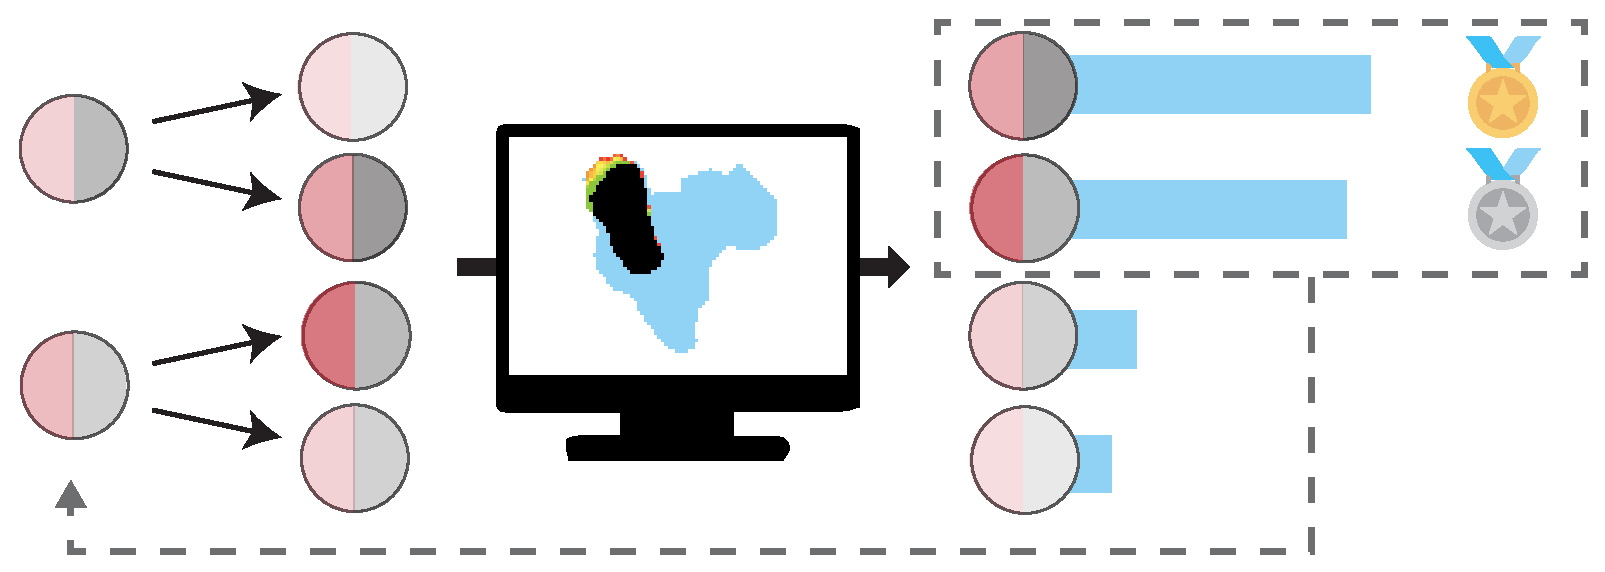
\includegraphics[width=6.5cm]{../cartoons/evo-setup.pdf}
	};
	\node[anchor = north west, text width = 1.9cm, align=justify] at (0.3,-0.4){
		1. Proliferation:\\mutate \textcolor{red!70!white}{$\text{max}_\text{act}$}, \textcolor{gray}{$\lambda_\text{act}$} in offspring
	};
	\node[anchor = north west, text width = 1.6cm, align=justify] at (2.45,-0.4){
		2. Simulation:\\ \textcolor{fitnessblue}{"fitness"} of the \\ migration
	};
	\node[anchor = north west, text width = 2.65cm, align=justify] at (4.3,-0.4){
		3. Selection: "fittest" searchers survive for the next generation
	};
	\node[anchor = north west, text width = 7cm] at (0.3,-4) {
		$ \textcolor{fitnessblue}{\text{fitness (cell)}} = \begin{cases}
			0 & \text{if cell breaks} \\
			\text{(covered area) / (cell area)} & \text{otherwise}
		\end{cases}$
	};
	\draw (0.3,-4) rectangle +(7,-0.85);
		
	\node[anchor = north west] at (0,0) {\figf A};		
\end{scope}


\begin{scope}[xshift=7.5cm]
	\node[anchor = north west] at (0,0) {
		\includegraphics{../plots/F2panelB.pdf}
	};
	
	
	\node[anchor = north west] at (0,0) {\figf B};		
\end{scope}

\begin{scope}[xshift=12cm]
	\node[anchor = north west] at (0,0) {
		\includegraphics{../plots/F2panelC.pdf}
	};
	
	
	\node[anchor = north west] at (0,0) {\figf C};		
\end{scope}



\end{tikzpicture}

\end{document}
